\documentclass[12pt]{article}
\author{Lawrence Liu}
\usepackage{subcaption}
\usepackage{graphicx}
\usepackage{amsmath}
\usepackage{pdfpages}
\newcommand{\Laplace}{\mathscr{L}}
\setlength{\parskip}{\baselineskip}%
\setlength{\parindent}{0pt}%
\usepackage{xcolor}
\usepackage{listings}
%\definecolor{backcolour}{rgb}{0.95,0.95,0.92}
\usepackage{amssymb}
\usepackage[T1]{fontenc}
\usepackage{beramono}%\lstdefinestyle{mystyle}{
%    backgroundcolor=\color{backcolour}}
%\lstset{style=mystyle}
%\usepackage[usenames,dvipsnames]{xcolor}%%
%% Julia definition (c) 2014 Jubobs
%%



\title{ECE 133A HW 6}
\begin{document}
\maketitle
\section*{Exercise A11.8}
\subsection*{(c)}
We have that 
$$R_11=1$$
And thus 
$$R_{1,2:3}=[0,1]$$
Thus now we need to compute the cholensky factorization of 
$$\begin{bmatrix}
    1 & 1\\
    1 & a
\end{bmatrix}-\begin{bmatrix}
    0 & 0\\
    0 & 1
\end{bmatrix}=\begin{bmatrix}
    1 & 1\\
    1 & a-1
\end{bmatrix}$$
Thus we have that 
$$R_{22}=1$$
And thus we have that 
$$R_{23}=1$$
And thus we have that
$$R_{33}=\sqrt{a-2}$$
Thus we have that A is positive definite if and only if $a\geq2$, and if it 
exists we have
$$R=\begin{bmatrix}
    1 & 0 & 1\\
    0 & 1 & 1\\
    0 & 0 & \sqrt{a-2}
\end{bmatrix}$$
\subsection*{(e)}
We have that 
$$R_11=\sqrt{a}$$
thus we must have that $a\geq 0$, and thus we also have that 
$$R_{1,2:3}=[\frac{1}{\sqrt{a}},0]$$
Therefore we have that we want to find the cholesky factorization of
of 
$$\begin{bmatrix}
    -a & 1\\
    1 & a
\end{bmatrix}-\begin{bmatrix}
    \frac{1}{a} & 0\\
    0 & 0
\end{bmatrix}=\begin{bmatrix}
    -a-\frac{1}{a} & 1\\
    1 & a
\end{bmatrix}$$
This cannot be factorized since we already have 
that $a\geq 0$ and thus we have that $-a-\frac{1}{a}\leq 0$. Thus we have
that A is not positive definite.
\subsection*{(h)}
We have that 
$$R_11=1$$
And thus
$$R_{1,2:3}=\frac{1}{1}A_{1,2:3}=[1,1]$$
Thus we have that we want to find the cholesky factorization of
$$\begin{bmatrix}
    a & a\\
    a & 2
\end{bmatrix}-\begin{bmatrix}
    1 & 1\\
    1 & 1
\end{bmatrix}=\begin{bmatrix}
    a-1 & a-1\\
    a-1 & 1
\end{bmatrix}$$
Thus we have that
$$R_{22}=\sqrt{a-1}$$
And thus we have that
$$R_{23}=\frac{a-1}{\sqrt{a-1}}=\sqrt{a-1}$$
Thus in order for these to exist we must have that $a\geq 1$, and thus we have
that 
$$R_{33}=\sqrt{1-a+1}=\sqrt{2-a}$$
This exists if $a\leq 2$ Therefore we have that 
A is positive definite if and only if $1\leq a\leq 2$, and if it exists we have
that 
$$R=\begin{bmatrix}
    1 & 1 & 1\\
    0 & \sqrt{a-1} & \sqrt{a-1}\\
    0 & 0 & \sqrt{2-a}
\end{bmatrix}$$
\section*{A11.14}
\subsection*{(a)}
We have that the cholensky factorization of $B$
$$B=R_B^T R_B$$
is of the form of  
$$R_B=\begin{bmatrix}
    R & v\\
    0 & v_{n+1}
\end{bmatrix}$$
Now we need to solve for $v$ and $v_{n+1}$, we have that
\begin{align*}
R_B^t R_B&=\begin{bmatrix}
    R^T & 0\\
    v^T & v_{n+1}
\end{bmatrix}\begin{bmatrix}
    R & v\\
    0 & v_{n+1}
\end{bmatrix}\\
&=\begin{bmatrix}
    R^T R & R^Tv\\
    v^TR & v^Tv+v_{n+1}^2
\end{bmatrix}
\end{align*}
Thus we have that 
$$v=R^{-T}u$$
and 
$$v_{n+1}^2=1-u^TA^{-1}u$$
and thus we have that
$$\boxed{
    R_B=\begin{bmatrix}
        R & R^{-T}u\\
        0 & \sqrt{1-u^TA^{-1}u}
    \end{bmatrix}
}$$
\subsection*{(b)}
To solve for $v$, since $R$ is a upper triangular matrix, we can just use
forward substitution to solve for $v$, which will cost us $n^2$ flops, 
then to solve for $v_{n+1}$ we take the dot product of $v$ with itself,
which will cost us $2n-1$ flops, and then subtract one and take the square 
root, which will cost us $2$ flops, thus we have that the total cost is
$\boxed{n^2+2n+1}$ flops.
\section*{Exercise A14.8}
\begin{verbatim}
using LinearAlgebra
using PyPlot

include("logistic_gn.jl")

function g(alpha,beta,t,y)
    # g= sum (y_i-e^(alpha*t_i+beta))/(1+e^(alpha*t_i+beta))^2

    g =zeros(length(t))
    for i in 1:length(t)
        g[i]= ((exp(alpha*t[i]+beta))/(1+exp(alpha*t[i]+beta)))-y[i]
    end
    return g
end

function Jacobian_g(alpha,beta,t,y)
    #dg/dalpha=-(2*t*((e^beta*y_i-e^beta)*e^(t*alpha)+y_i)*e^(t*alpha+beta))/(e^(t*alpha+beta)+1)^3
    #dg/dbeta=-(2*((e^(alpha*t)*y_i-e^(alpha*t))*e^beta+y_i)*e^(beta+alpha*t))/(e^(beta+alpha*t)+1)^3

    J = zeros(length(t),2)
    for i in 1:length(t)
        t_i=t[i]
        y_i=y[i]
        J[i,1] += (t_i*exp(t_i*alpha+beta))/(exp(t_i*alpha+beta)+1)^2
        J[i,2] += exp(beta+alpha*t_i)/(exp(beta+alpha*t_i)+1)^2
    end
    return J
end

function main()

    params=[0,0]

    for i=1:10
        #using newton's method to optimize g 
        alpha=params[1]
        beta=params[2]
        g_= g(alpha,beta,t,y)
        J= Jacobian_g(alpha,beta,t,y)
        # println(sum(J.*(g_\J)))
        params=params.-inv(J'*J)*(J'*g_)
        delta_g=2*(transpose(J)*g_)

        if norm(delta_g)<=1e-6
            break
        end
    end
    println("alpha=",params[1])
    println("beta=",params[2])
    plot(t,y,"o")
    plot(t,exp.(params[1]*t.+params[2])./(ones(length(t))+exp.(params[1]*t.+params[2])))
    savefig("test.png")
    close()
end

main()
\end{verbatim}
We get that $\alpha=2.997$ and $\beta=-4.015$. Which results in the following
plot\\
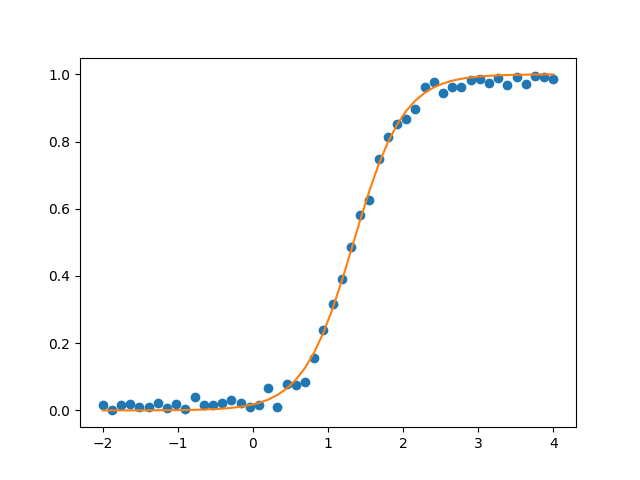
\includegraphics[width=\textwidth]{test.png}
\section*{Exercise A12.2}
\subsection*{(a)}
We want to find the two values of $t$, $t_1$ and $t_2$, such that
$n(t_1)=n(t_2)=2$, we can write the newton's update as 
\begin{multline*}
    \begin{bmatrix}
    t_1^{(k+1)}\\
    t_2^{(k+1)}
\end{bmatrix}=\begin{bmatrix}
    t_1^{(k)}\\
    t_2^{(k)}
\end{bmatrix}\\-\begin{bmatrix}
    -20t_1e^{-2t_1^{(k)}}-e^{-t_1^{(k)}}+10e^{-t_1^{(k)}} & 0\\
    0 & -20t_2e^{-2t_2^{(k)}}-e^{-t_2^{(k)}}+10e^{-t_2^{(k)}}
\end{bmatrix}^{-1}\begin{bmatrix}
    10t_1e^{-2t_1^{(k)}}+e^{-t_1^{(k)}}-2\\
    10t_2e^{-2t_2^{(k)}}+e^{-t_2^{(k)}}-2
\end{bmatrix}
\end{multline*}
We can compute this newton's method in Julia with the following code:
\begin{verbatim}
    using LinearAlgebra

function n(T)
    n=zeros(length(T))
    for i in 1:length(T)
        t=T[i]
        n[i]=10*t*exp(-2*t)+exp(-t)-2
    end
    return n
end

function dn(T)
    dn=zeros(length(T))
    for i in 1:length(T)
        t=T[i]
        dn[i]=10*exp(-2*t)*(1-2*t)-exp(-t)
    end
    return dn
end

t_1=0
t_2=1

let T=[t_1,t_2]
    #newton's method 
    thresh=0.00001
    while norm(n(T))>thresh
        T=T.-n(T)./dn(T)
    end
    println(T)
    println(n(T).+[2,2])
end
\end{verbatim}
With which we get
$t_1=0.15661093823882483$, and $t_2=0.8383819928969031$
\subsection*{(b)}
for a value to reach the maximum, we would want its derivative to go to zero, 
so then we have that the newton's update to find $t_{\text{max}}$
$$
    t_{\text{max}}^{(k+1)}=
    t_{\text{max}}^{(k)}-\frac{10e^{-2t_{\text{max}}^{(k)}}(1-2t_{\text{max}}^{(k)})+e^{-t_{\text{max}}^{(k)}}}
    {e^{-2t_{\text{max}}^{(k)}}(e^{t_{\text{max}}^{(k)}}+40t_{\text{max}}^{(k)}-40)}
$$
With the following code in addition to the code we wrote for part a we get that 
$t_{\text{max}}=\boxed{0.4236255212307657}$
\begin{verbatim}
    function d2n(T)
    d2n=zeros(length(T))
    for i in 1:length(T)
        t=T[i]
        d2n[i]=exp(-2*t)*(exp(t)+40*t-40)
    end
    return d2n
end

let t_max=[0]
    thresh=0.00001
    while norm(dn(t_max))>thresh
        t_max=t_max.-dn(t_max)./d2n(t_max)
    end
    println("t_max=",t_max[1])
    println("n(t_max)=",n(t_max)[1]+2)
end
\end{verbatim}



\end{document}


